\documentclass[landscape,fleqno]{foils}

\usepackage{ae}
%\usepackage{hyperref}
%\usepackage{thumbpdf}
\usepackage{graphicx}
\usepackage{color}
\usepackage[left=1cm,right=1cm,top=2cm,bottom=2cm]{geometry}
% \usepackage[display]{texpower}
%\usepackage{psfrag}
\usepackage{ragged2e}
\usepackage{amstext}
\usepackage{xspace}
\usepackage{fancyvrb}
\usepackage{amsmath}
\usepackage{url}
\usepackage{pause}

\newcommand{\figfigure}[2]{%
  \begin{psfrags}%
  \input #2.eps_t%
  \includegraphics[width=#1]{#2.eps}%
  \end{psfrags}%
}

\newcommand{\stitle}[1]{{\color{blue}\Large #1\par\vspace*{10pt}\hrule}}
\newcommand{\cstitle}[1]{{\centering\color{blue}\Large #1\par\vspace*{10pt}\hrule}}

\setlength{\columnsep}{0.5cm}
\setlength{\columnseprule}{0.4pt}

\renewcommand{\emph}[1]{\textcolor{red}{\bf #1}}

\newcommand{\igraph}{\texttt{{igraph}}\xspace}

\DefineVerbatimEnvironment{Myverb}{Verbatim}
{gobble=2,numbers=left,numbersep=5mm,frame=lines,fontsize=\small}

\newenvironment{narrow}[2]{%
  \begin{list}{}{%
      \setlength{\topsep}{0pt}%
      \setlength{\leftmargin}{#1}%
      \setlength{\rightmargin}{#2}%
      \setlength{\listparindent}{\parindent}%
      \setlength{\itemindent}{\parindent}%
      \setlength{\parsep}{\parskip}}%
    \item[]}{\end{list}}

\begin{document}

\RaggedRight
% \color{white}
% \pagecolor{black}
\fvset{fontsize=\small}
\fvset{commandchars=\\\{\}}
\definecolor{grey}{gray}{0.75}
\fvset{frame=single, numbers=left, rulecolor=\color{grey}}

\MyLogo{\color{black}Practical statistical network analysis -- WU Wien}

\thispagestyle{empty}
\vspace*{1cm}
{\centering
\hrule
\Large
\vspace*{1cm}
{\bf Practical statistical network analysis\\ (with \emph{R} and \igraph)}
\vspace*{1cm}
\par
\hrule
\par
\vspace*{2cm}
\normalsize G\'abor Cs\'ardi\\
\small \verb+csardi@rmki.kfki.hu+
\par
\vspace*{1.5cm}
Department of Biophysics, 
KFKI Research Institute for Nuclear and Particle Physics of the\\
Hungarian Academy of Sciences, Budapest, Hungary\\[15pt]
Currently at \\Department of Medical Genetics, \\
University of Lausanne, Lausanne, Switzerland\\
}

\newpage
\stitle{What is a network (or graph)?}
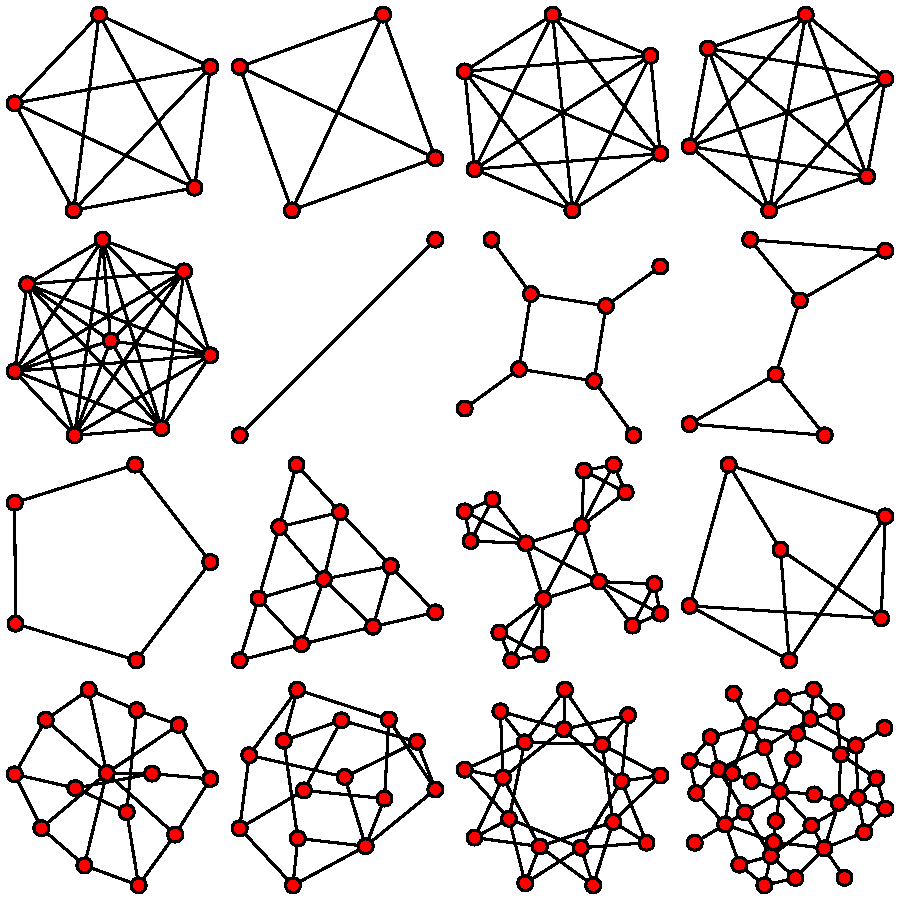
\includegraphics[width=0.5\textwidth]{frplots}

\newpage
\cstitle{What is a network (or graph)?}
\begin{center}
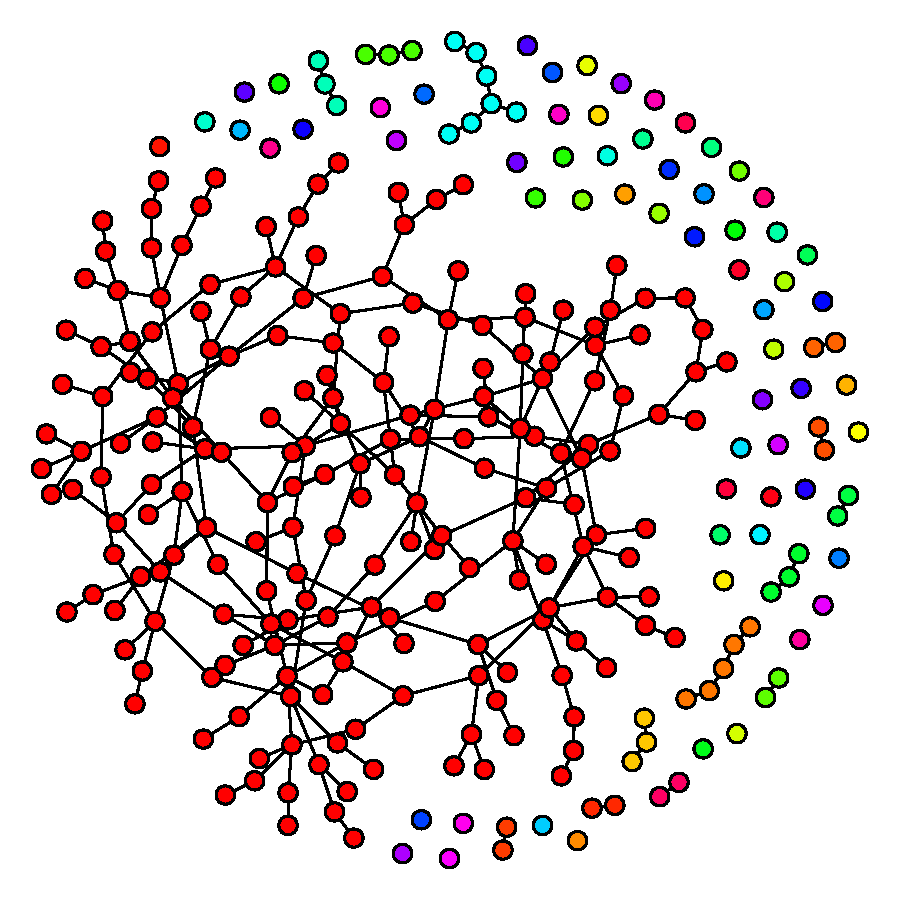
\includegraphics[width=0.6\textwidth]{ercomps}
\end{center}

\newpage
\cstitle{What is a network (or graph)?}
\begin{center}
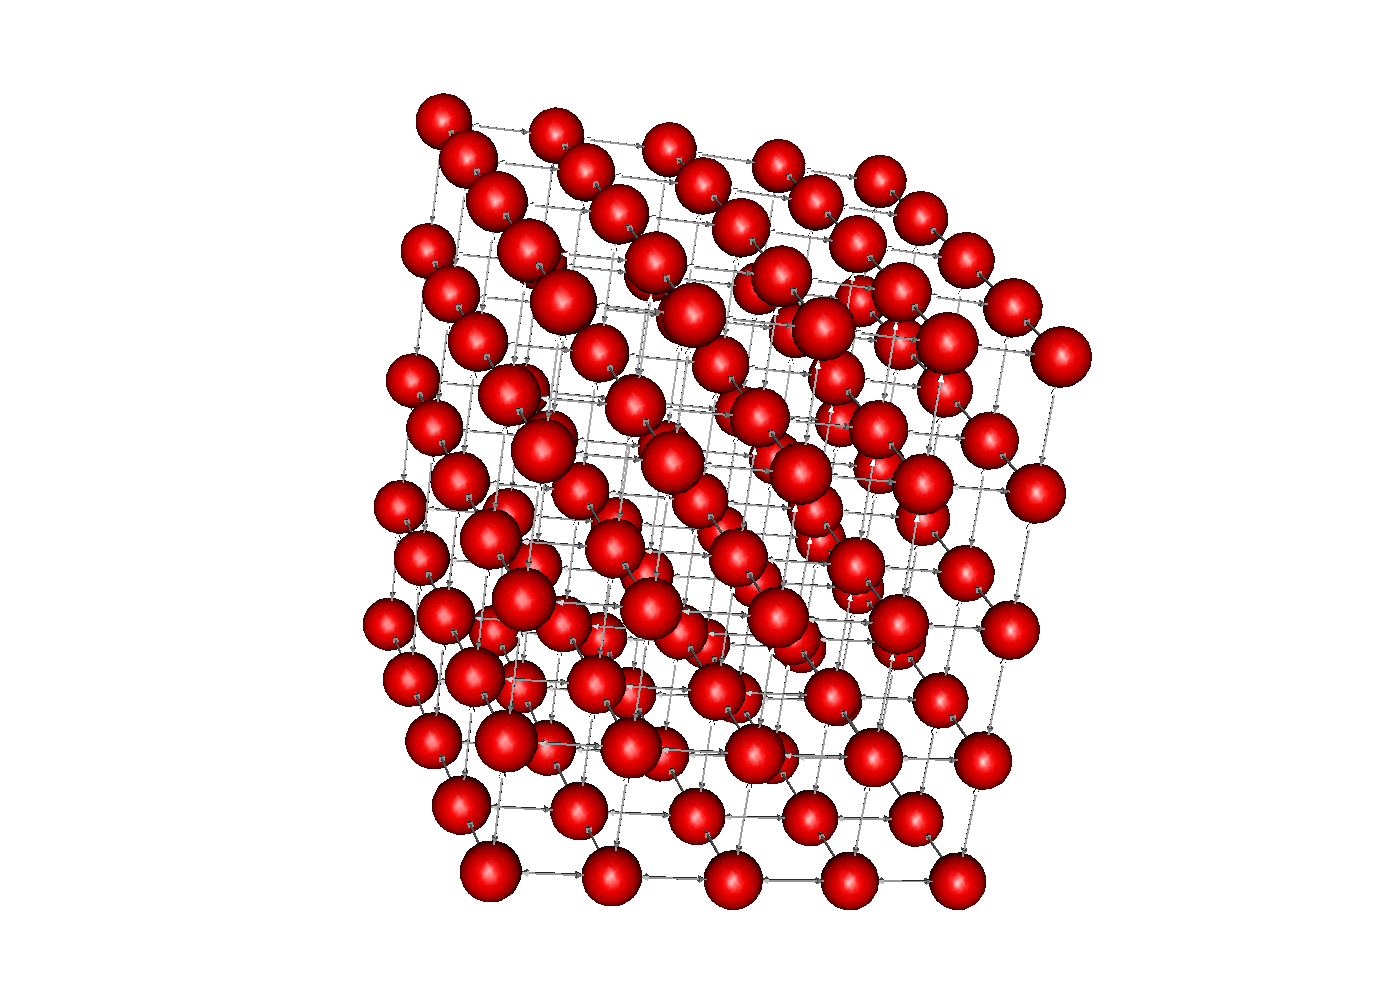
\includegraphics[width=0.8\textwidth]{3dplot}
\end{center}

\newpage
\cstitle{What is a graph?}
\begin{itemize}
\item Binary relation (=\emph{edges}) between elements of a set
  (=\emph{vertices}). \pause\\[-15pt]
\item E.g. 
  \begin{align} 
    \text{vertices} & =\{A,B,C,D,E\} \nonumber\\
    \text{edges}    & =( \{A,B\},\{A,C\},\{B,C\}, \{C,E\} ). \nonumber
  \end{align} \pause
\item It is ``better'' to draw it:
  \begin{center}
    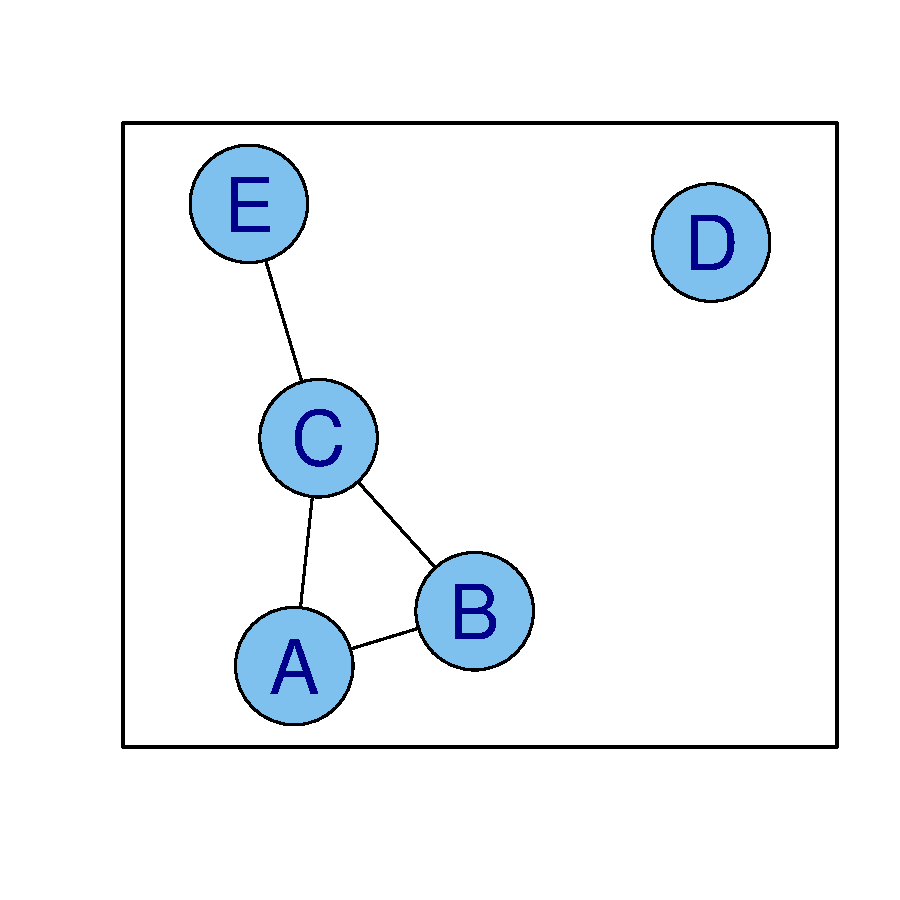
\includegraphics[width=0.25\textwidth]{small1} \pause
    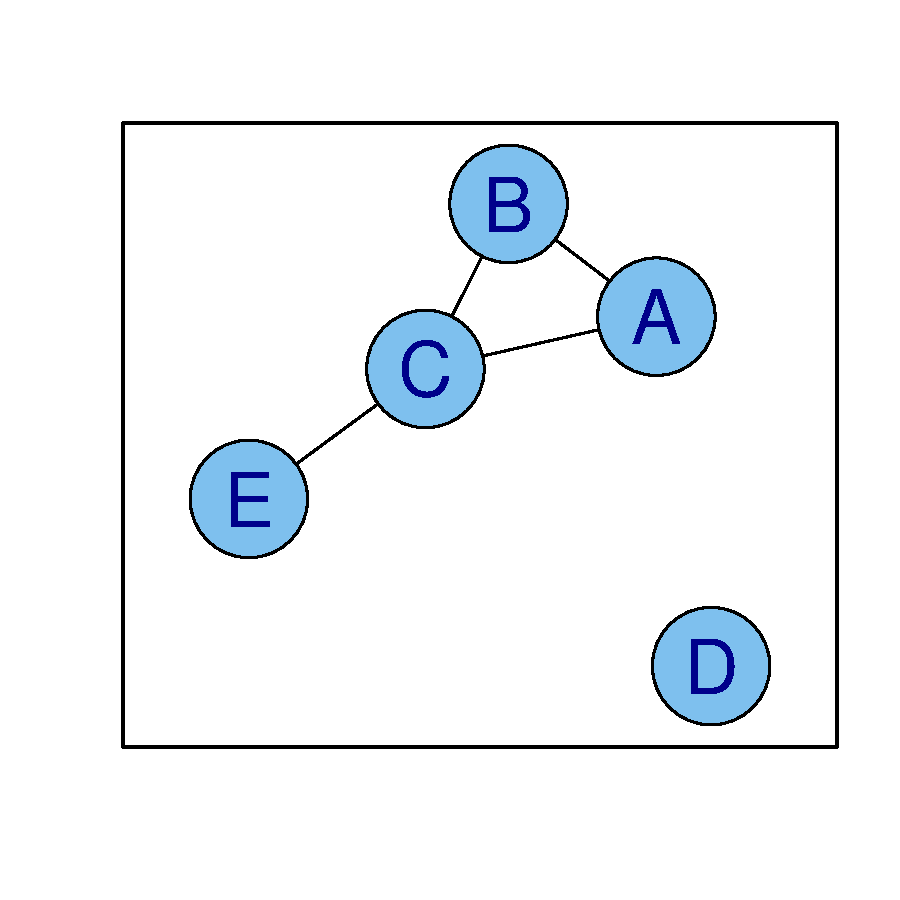
\includegraphics[width=0.25\textwidth]{small2}
  \end{center}
\end{itemize}

\newpage
\cstitle{Undirected and directed graphs}
\begin{itemize}
\item If the pairs are unordered, then the graph is undirected:

  \begin{minipage}{0.7\textwidth}
    \begin{align} 
      \text{vertices} & =\{A,B,C,D,E\} \nonumber\\
      \text{edges}    & =( \{A,B\},\{A,C\},\{B,C\},\{C,E\} ). \nonumber
    \end{align}
  \end{minipage}\begin{minipage}{0.3\textwidth}
    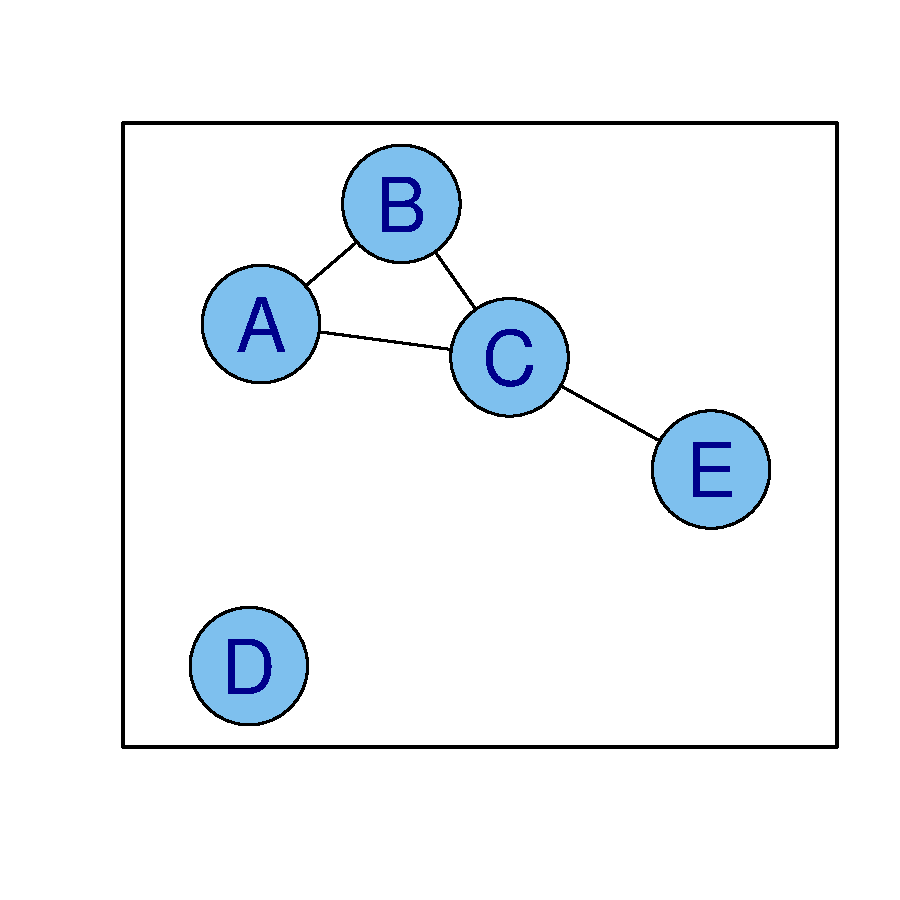
\includegraphics[width=0.8\textwidth]{small3}
  \end{minipage}\pause

\item Otherwise it is directed:

  \begin{minipage}{0.7\textwidth}
    \begin{align} 
      \text{vertices} & =\{A,B,C,D,E\} \nonumber\\
      \text{edges}    & =( (A,B),(A,C),(B,C),(C,E) ). \nonumber
    \end{align}
  \end{minipage}\begin{minipage}{0.3\textwidth}
    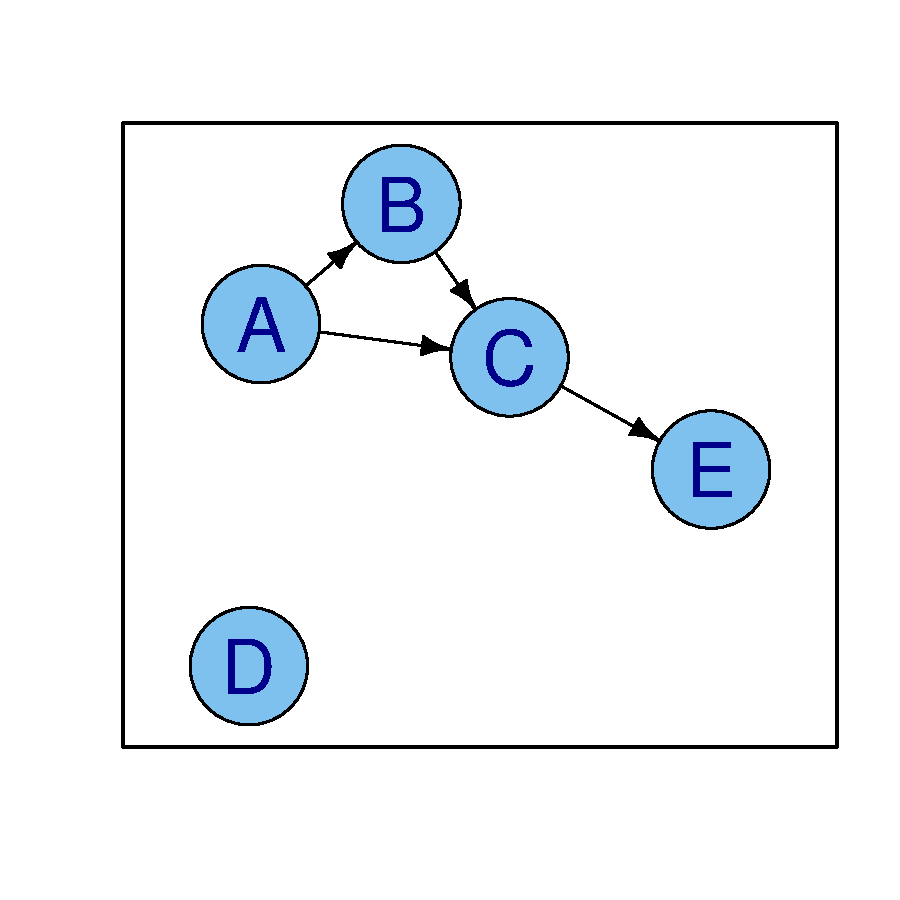
\includegraphics[width=0.8\textwidth]{small4}
  \end{minipage}
\end{itemize}

\newpage
\stitle{The \igraph ``package''}

\begin{narrow}{0cm}{10cm}
\begin{itemize}
\item For classic graph theory and network science.
\item Core functionality is implemented as a C library.
\item High level interfaces from \emph{R} and \emph{Python}.
\item GNU GPL.
\item \url{http://igraph.sf.net}
\end{itemize}
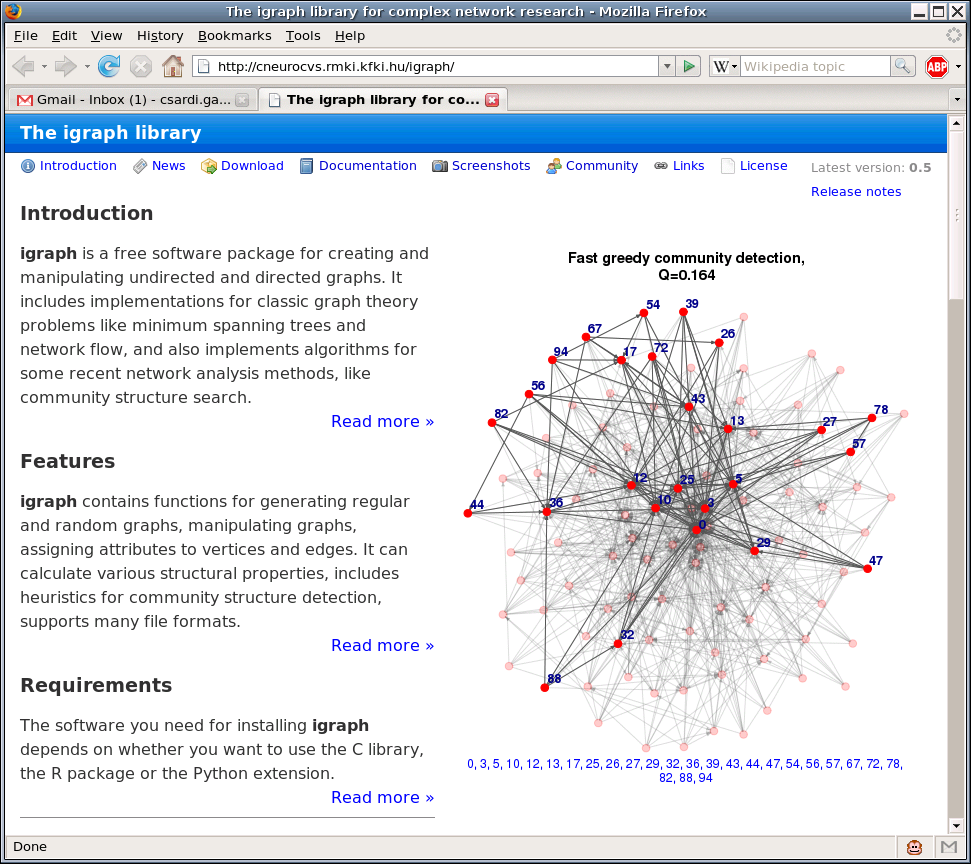
\includegraphics[width=0.45\textwidth]{homepage}
\end{narrow}

\newpage
\stitle{Vertex and edge ids}
\begin{narrow}{0cm}{12cm}
\begin{itemize}
\item Vertices are always numbered from zero (!).
\item Numbering is continual, form 0 to $|V|-1$. \pause
\item We have to ``translate'' vertex names to ids: 
\begin{align} 
  V & =\{A,B,C,D,E\} \nonumber\\
  E & =( (A,B),(A,C),(B,C),(C,E) ). \nonumber\\
  A & =0, B=1, C=2, D=3, E=4. \nonumber
\end{align} \pause
\begin{Myverb}
  > g <- graph( c(0,1, 0,2, 1,2, 2,4), n=5 )
\end{Myverb}
\end{itemize}
\end{narrow}

\newpage
\stitle{Creating \igraph graphs}
% Giving the edges
% igraph objects
% is.igraph, is.directed, vcount, ecount, summary
\begin{narrow}{0cm}{12cm}
\begin{itemize}
\item \igraph objects \pause
\item \verb+print()+, \verb+summary()+, \verb+is.igraph()+ \pause
\item \verb+is.directed()+, \verb+vcount()+, \verb+ecount()+
\end{itemize}
\begin{Myverb}
  > g <- graph( c(0,1, 0,2, 1,2, 2,4), n=5 )
  > g
  Vertices: 5 
  Edges: 4 
  Directed: TRUE 
  Edges:
          
  [0] 0 -> 1
  [1] 0 -> 2
  [2] 1 -> 2
  [3] 2 -> 4
\end{Myverb}
\end{narrow}

\newpage
\stitle{Visualization}
\begin{narrow}{0cm}{12cm}
\begin{Myverb}
  > g <- graph.tree(40, 4)
  > plot(g)
  > plot(g, layout=layout.circle)
\end{Myverb}
\vspace*{-2cm} \pause
\begin{Myverb}
  # Force directed layouts
  > plot(g, layout=layout.fruchterman.reingold)
  > plot(g, layout=layout.graphopt)
  > plot(g, layout=layout.kamada.kawai)
\end{Myverb}
\vspace*{-2cm} \pause
\begin{Myverb}
  # Interactive
  > tkplot(g, layout=layout.kamada.kawai)
  > l <- layout=layout.kamada.kawai(g)
\end{Myverb}
\vspace*{-2cm} \pause
\begin{Myverb}
  # 3D
  > rglplot(g, layout=l)
\end{Myverb}
\vspace*{-2cm} \pause
\begin{Myverb}
  # Visual properties
  > plot(g, layout=l, vertex.color="cyan")
\end{Myverb}
\end{narrow}

\newpage
\stitle{Simple graphs}
\begin{narrow}{0cm}{15cm}
\begin{itemize}
\item \igraph can handle multi-graphs:
  \begin{align} 
    V & =\{A,B,C,D,E\} \nonumber\\
    E & =( (AB),(AB),(AC),(BC),(CE) ). \nonumber
  \end{align}
  \begin{Myverb}
  > g <- graph( c(0,1,0,1, 0,2, 1,2, 3,4), n=5 )
  > g
  Vertices: 5 
  Edges: 5 
  Directed: TRUE 
  Edges:
          
  [0] 0 -> 1
  [1] 0 -> 1
  [2] 0 -> 2
  [3] 1 -> 2
  [4] 3 -> 4
  \end{Myverb}
\end{itemize}
\end{narrow}

\newpage
\stitle{Simple graphs}
\begin{narrow}{0cm}{15cm}
\begin{itemize}
\item \igraph can handle loop-edges:
  \begin{align} 
    V & =\{A,B,C,D,E\} \nonumber\\
    E & =( (AA),(AB),(AC),(BC),(CE) ). \nonumber
  \end{align}
  \begin{Myverb}
  > g <- graph( c(0,0,0,1, 0,2, 1,2, 3,4), n=5 )
  > g
  Vertices: 5 
  Edges: 5 
  Directed: TRUE 
  Edges:
          
  [0] 0 -> 0
  [1] 0 -> 1
  [2] 0 -> 2
  [3] 1 -> 2
  [4] 3 -> 4
  \end{Myverb}
\end{itemize}
\end{narrow}

\newpage
\stitle{Creating (more) \igraph graphs}
\begin{narrow}{0cm}{15cm}
\begin{Myverb}
 > el <- scan("lesmis.txt")
 > el <- matrix(el, byrow=TRUE, nc=2)
 > gmis <- graph.edgelist(el, dir=FALSE)
 > summary(gmis)
\end{Myverb}
\end{narrow}

\newpage
\stitle{Naming vertices}
\begin{narrow}{0cm}{15cm}
\begin{Myverb}
 > V(gmis)$name
 > g <- graph.ring(10)
 > V(g)$name <- sample(letters, vcount(g))
\end{Myverb}
\end{narrow}
% From edge list, data frame
% graph.edgelist
% graph.data.frame

\newpage
\stitle{Creating (more) \igraph graphs}
\begin{narrow}{0cm}{15cm}
\begin{Myverb}
  # A simple undirected graph
  > g <- graph.formula( Alice-Bob-Cecil-Alice, 
      Daniel-Cecil-Eugene, Cecil-Gordon )
\end{Myverb}
\vspace*{-2cm} \pause
\begin{Myverb}
  # Another undirected graph, ":" notation
  > g2 <- graph.formula( Alice-Bob:Cecil:Daniel, 
      Cecil:Daniel-Eugene:Gordon )
\end{Myverb}
\vspace*{-2cm} \pause
\begin{Myverb}
  # A directed graph
  > g3 <- graph.formula( Alice +-+ Bob --+ Cecil 
      +-- Daniel, Eugene --+ Gordon:Helen )
\end{Myverb}
\vspace*{-2cm} \pause
\begin{Myverb}
  # A graph with isolate vertices
  > g4 <- graph.formula( Alice -- Bob -- Daniel, 
      Cecil:Gordon, Helen )
\end{Myverb}
\vspace*{-2cm} \pause
\begin{Myverb}
  # "Arrows" can be arbitrarily long
  > g5 <- graph.formula( Alice +---------+ Bob )
\end{Myverb}
\end{narrow}
% Formula notation

\newpage
\stitle{Vertex/Edge sets, attributes}
\begin{narrow}{0cm}{15cm}
\begin{itemize}
\item Assigning attributes:
  \texttt{set/get.graph/vertex/edge.attribute}. \pause\vspace*{-0.8cm}
\item \verb+V(g)+ and \verb+E(g)+. \pause
\item Smart indexing, e.g. \verb+V(g)[color=="white"]+ \pause
\item Easy access of attributes:
  \begin{Myverb}
  > g <- erdos.renyi.game(100, 1/100)
  > V(g)$color <- sample( c("red", "black"), 
                          vcount(g), rep=TRUE)
  > E(g)$color <- "grey"
  > red <- V(g)[ color == "red" ]
  > bl <- V(g)[ color == "black" ]
  > E(g)[ red %--% red ]$color <- "red"
  > E(g)[ bl  %--% bl ]$color <- "black"
  > plot(g, vertex.size=5, layout=
         layout.fruchterman.reingold)
\end{Myverb}
\end{itemize}
\end{narrow}

\newpage
\stitle{Creating (even) more graphs}
\begin{narrow}{0cm}{15cm}
\begin{itemize}
\item E.g. from \verb+.csv+ files.
\end{itemize}
\begin{Myverb}
  > traits <- read.csv("traits.csv", head=F)
  > relations <- read.csv("relations.csv", head=F)
  > orgnet <- graph.data.frame(relations)

  > traits[,1] <- sapply(strsplit(as.character
    (traits[,1]), split=" "), "[[", 1)
  > idx <- match(V(orgnet)$name, traits[,1])
  > V(orgnet)$gender <- as.character(traits[,3][idx])
  > V(orgnet)$age <- traits[,2][idx]
  
  > igraph.par("print.vertex.attributes", TRUE)
  > orgnet
\end{Myverb}
% $
\end{narrow}

\newpage
\stitle{Creating (even) more graphs}
\begin{narrow}{0cm}{15cm}
\begin{itemize}
\item From the web, e.g. Pajek files.
\end{itemize}
\begin{Myverb}
  > karate <- read.graph("http://cneurocvs.rmki.kfki.hu/igraph/karate.net",
                         format="pajek")
  > summary(karate)
  Vertices: 34 
  Edges: 78 
  Directed: FALSE 
  No graph attributes.
  No vertex attributes.
  No edge attributes.
\end{Myverb}
\end{narrow}

\newpage
\stitle{Graph representation}
\begin{narrow}{0cm}{15cm}
\begin{itemize}
\item There is no best format, everything depends on
  what kind of questions one wants to ask.
\begin{center}
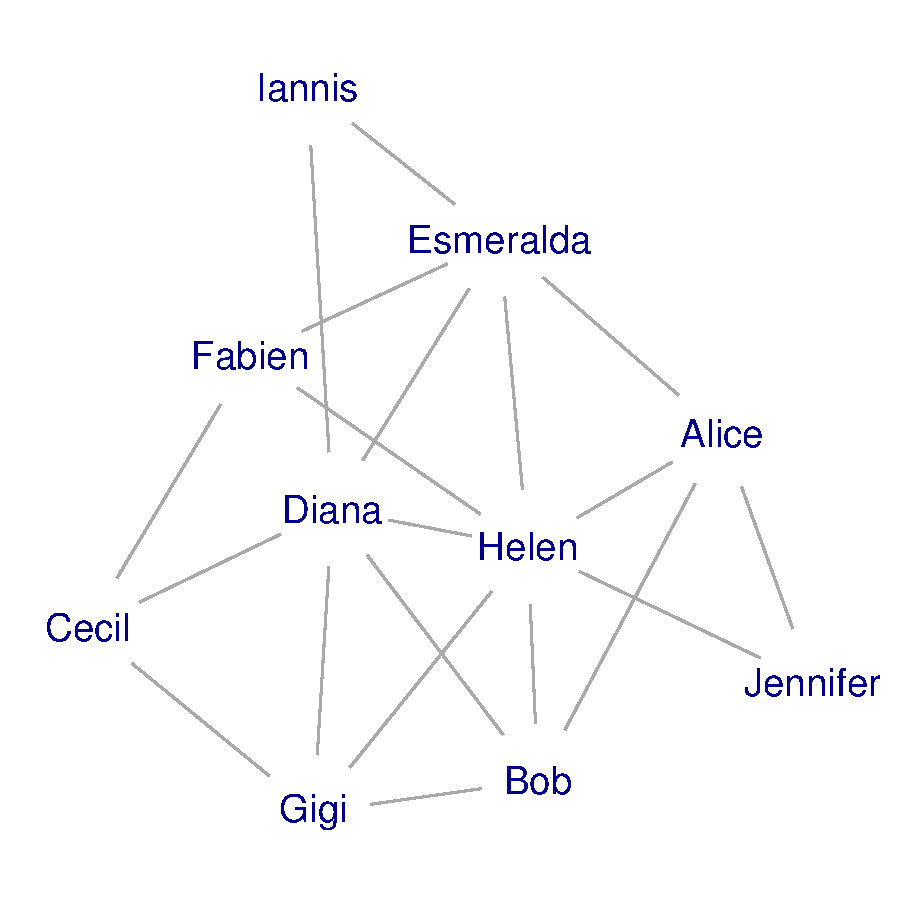
\includegraphics[width=0.45\textwidth]{example}
\end{center}
\end{itemize}
\end{narrow}

\newpage
\stitle{Graph representation}
\begin{narrow}{0cm}{15cm}
\begin{itemize}
\item Adjacency matrix. Good for questions like: is 'Alice' connected
  to 'Bob'?
\begin{center}
  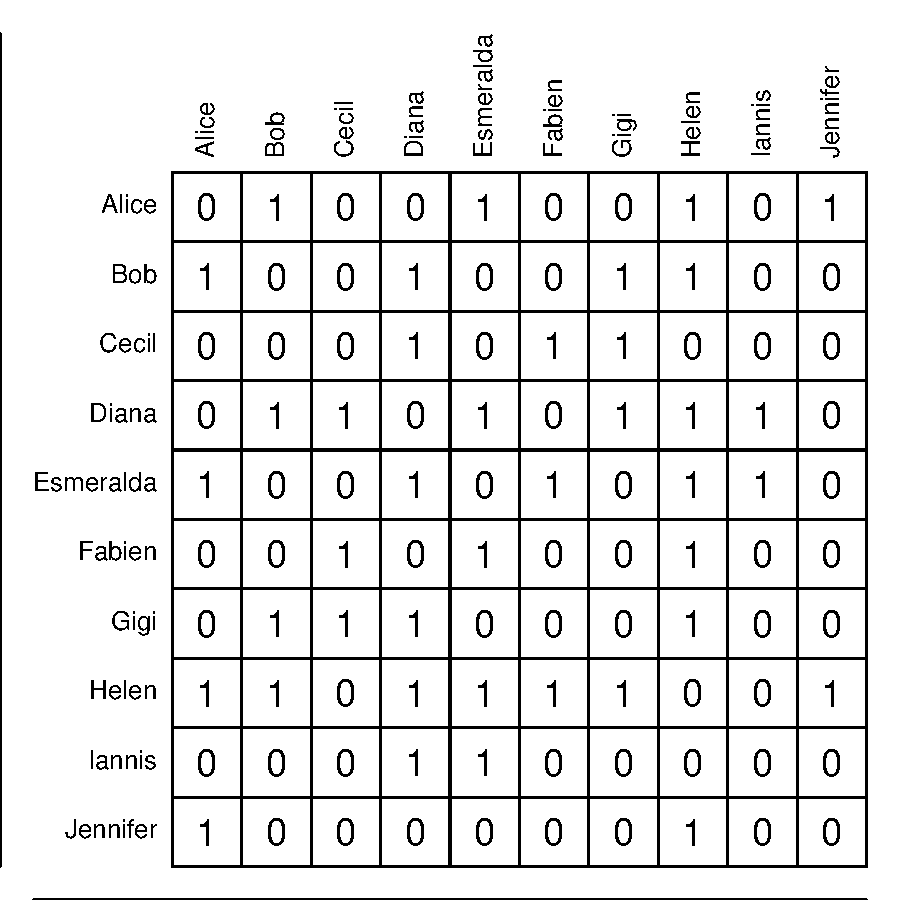
\includegraphics[width=0.45\textwidth]{adjacency}
\end{center}
\end{itemize}
\end{narrow}

\newpage
\stitle{Graph representation}
\begin{narrow}{0cm}{15cm}
\begin{itemize}
\item Edge list. Not really good for anything.
\begin{center}
  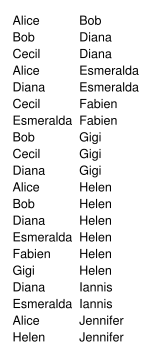
\includegraphics{edgelist}
\end{center}
\end{itemize}
\end{narrow}

\newpage
\stitle{Graph representation}
\begin{narrow}{0cm}{15cm}
\begin{itemize}
\item Adjacency lists. GQ: who are the neighbors of 'Alice'?
\begin{center}
  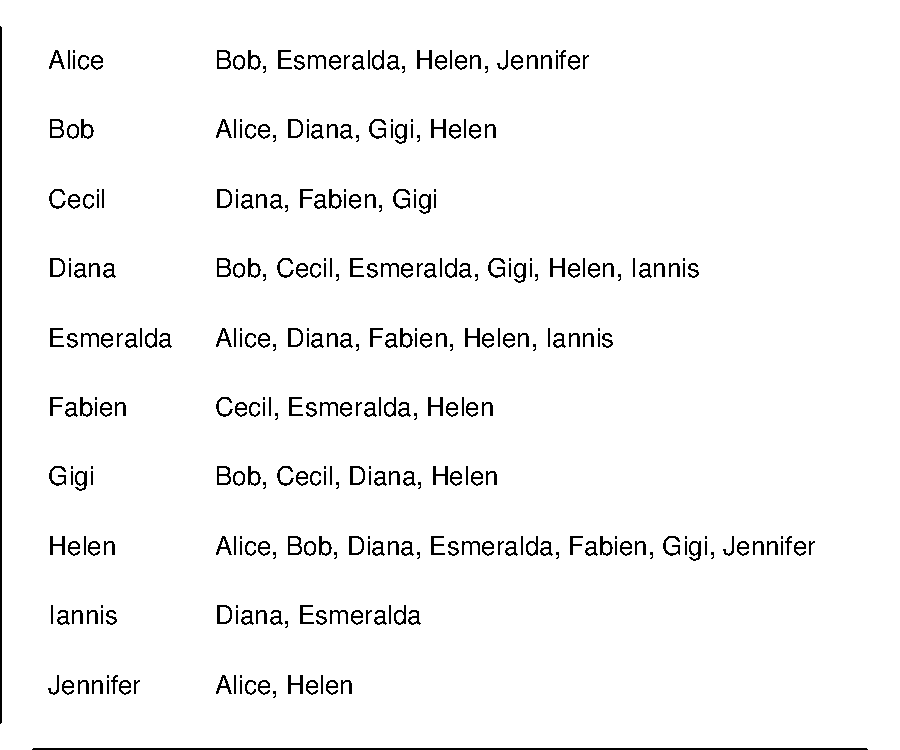
\includegraphics{adjlist}
\end{center}
\end{itemize}
\end{narrow}

\newpage
\stitle{Graph representation}
\begin{narrow}{0cm}{15cm}
\begin{itemize}
\item \igraph. Flat data structures, indexed edge lists. Easy to
  handle, good for many kind of questions.
\begin{center}
  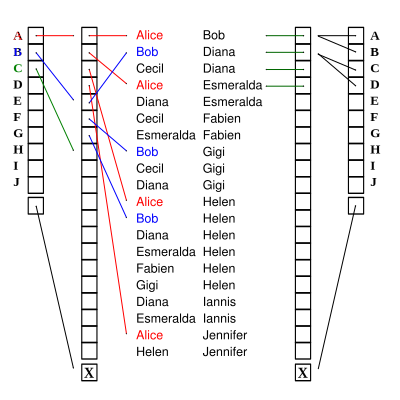
\includegraphics[width=0.45\textwidth]{igraph}
\end{center}
\end{itemize}
\end{narrow}
% Adjacency matrix, edge list, adjacency lists,
% igraph

\newpage
\stitle{Centrality in networks}
\begin{narrow}{0cm}{15cm}
\begin{itemize}
\item degree
\begin{center}
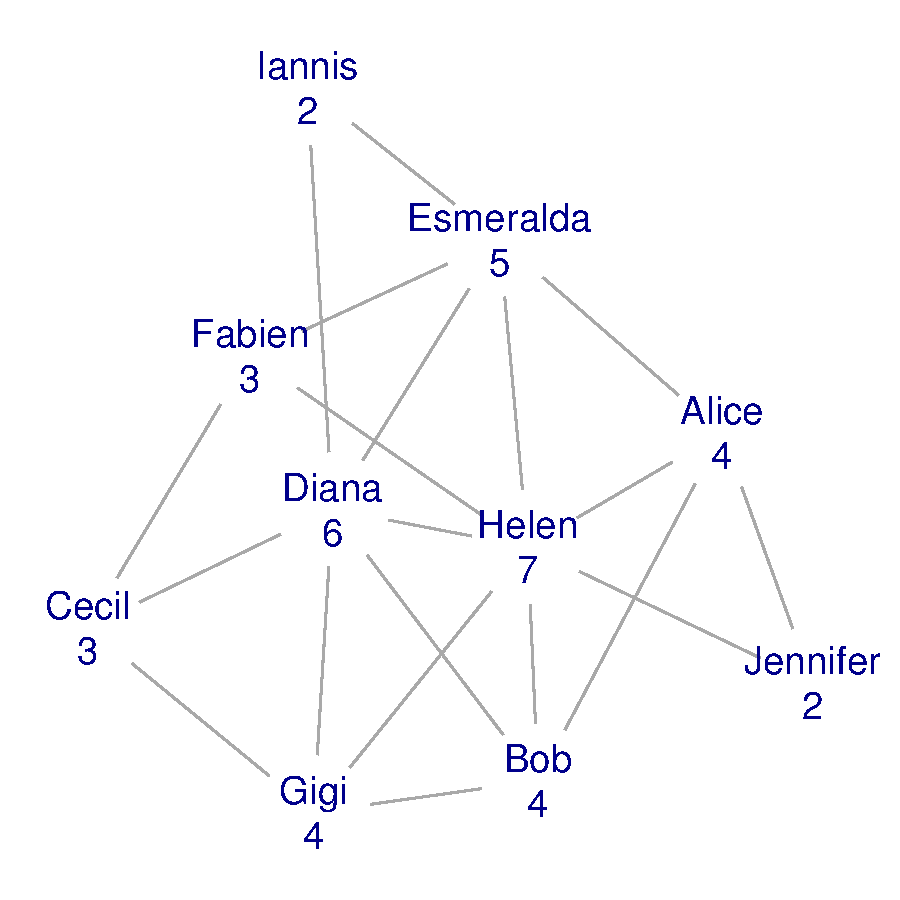
\includegraphics[width=0.45\textwidth]{ex-deg}
\end{center}
\end{itemize}
\end{narrow}

\newpage
\stitle{Centrality in networks}
\begin{narrow}{0cm}{15cm}
\begin{itemize}
\item closeness
  \[ C_v = \frac{|V|-1}{\sum_{i\ne v} d_{vi}} \]
\begin{center}
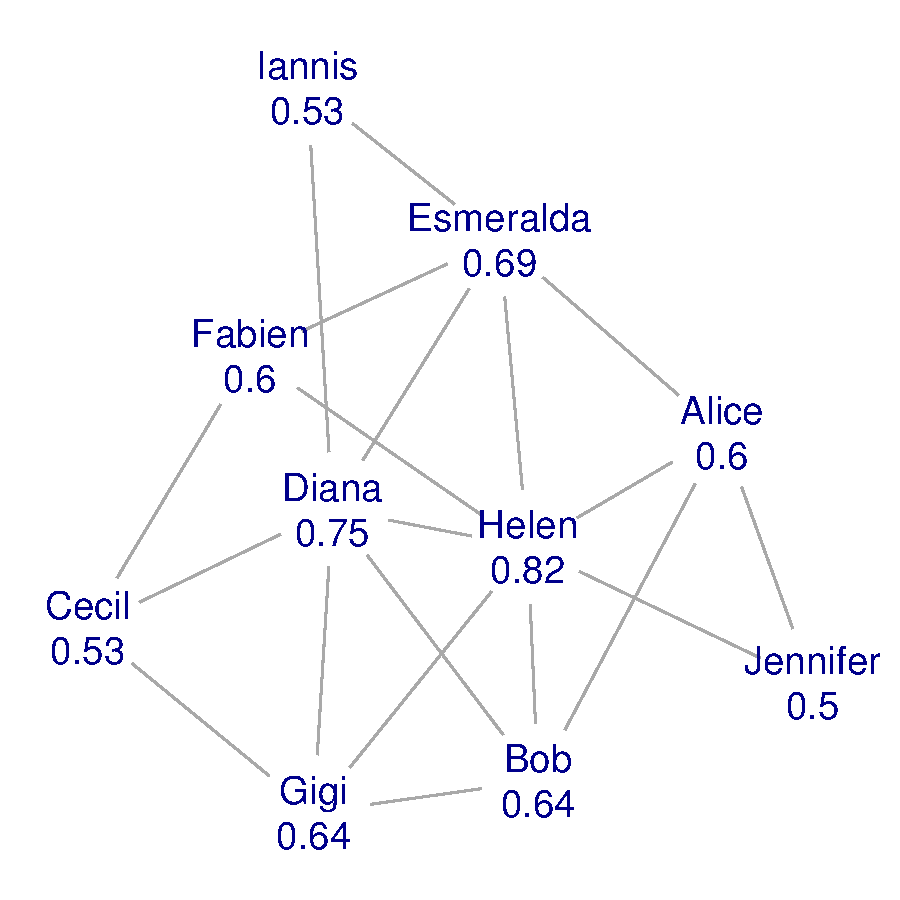
\includegraphics[width=0.45\textwidth]{ex-close}
\end{center}
\end{itemize}
\end{narrow}

\newpage
\stitle{Centrality in networks}
\begin{narrow}{0cm}{15cm}
\begin{itemize}
\item betweenness
  \[ B_v= \sum_{i\ne j, i\ne v, j\ne v} g_{ivj}/g_{ij} \]
\begin{center}
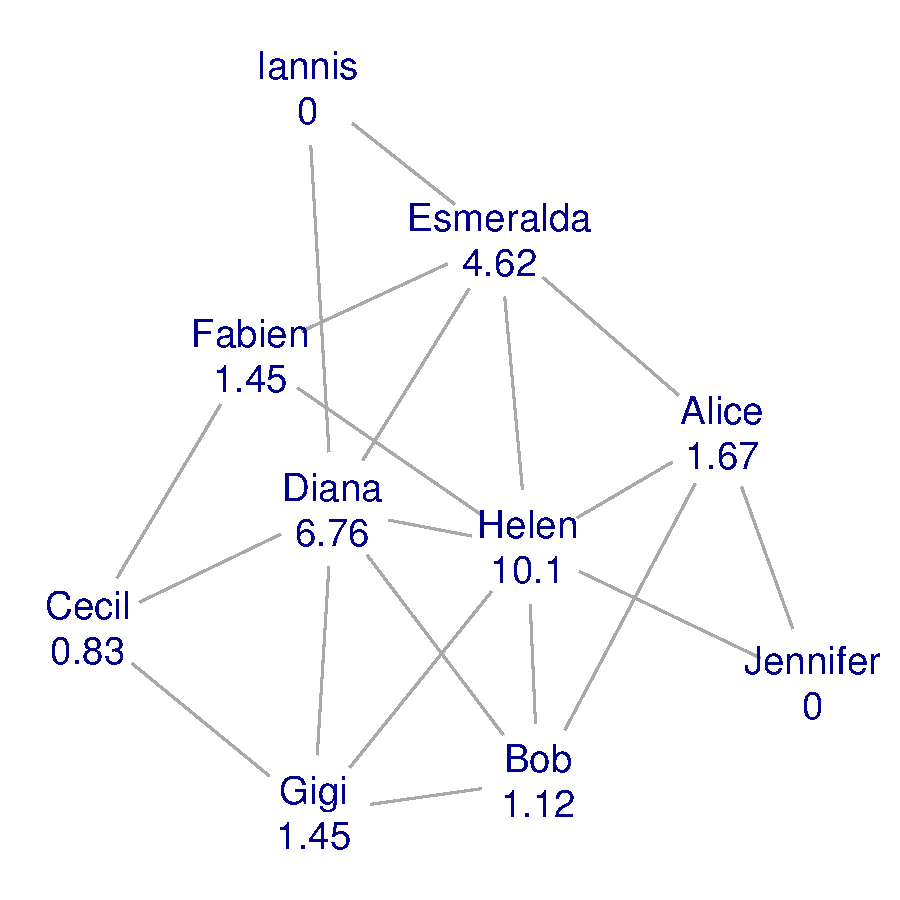
\includegraphics[width=0.45\textwidth]{ex-betw}
\end{center}
\end{itemize}
\end{narrow}

\newpage
\stitle{Centrality in networks}
\begin{narrow}{0cm}{15cm}
\begin{itemize}
\item eigenvector centrality
\[ E_v = \frac{1}{\lambda} \sum_{i=1}^{|V|} A_{iv} E_i, 
   \quad Ax=\lambda x \]
\begin{center}
\vspace*{-1cm}
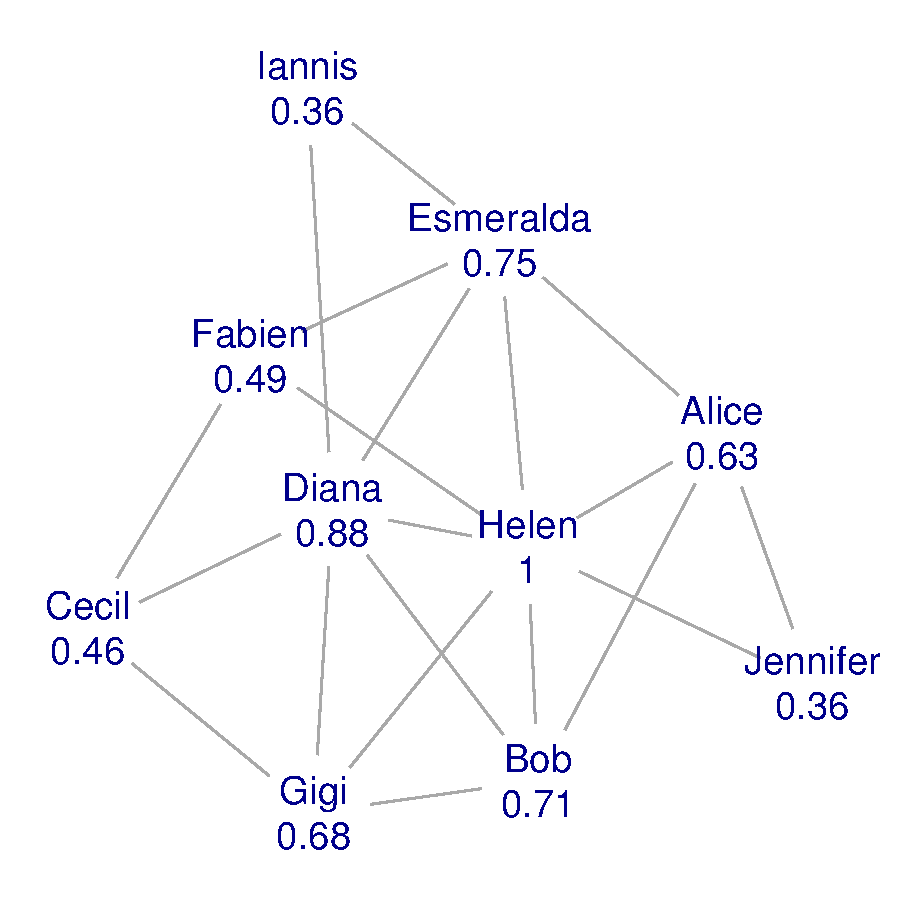
\includegraphics[width=0.45\textwidth]{ex-ev}
\end{center}
\end{itemize}
\end{narrow}

\newpage
\stitle{Centrality in networks}
\begin{narrow}{0cm}{15cm}
\begin{itemize}
\item page rank
\[ E_v =  \frac{1-d}{|V|} + d \sum_{i=1}^{|V|} A_{iv} E_i \]
\begin{center}
\vspace*{-1cm}
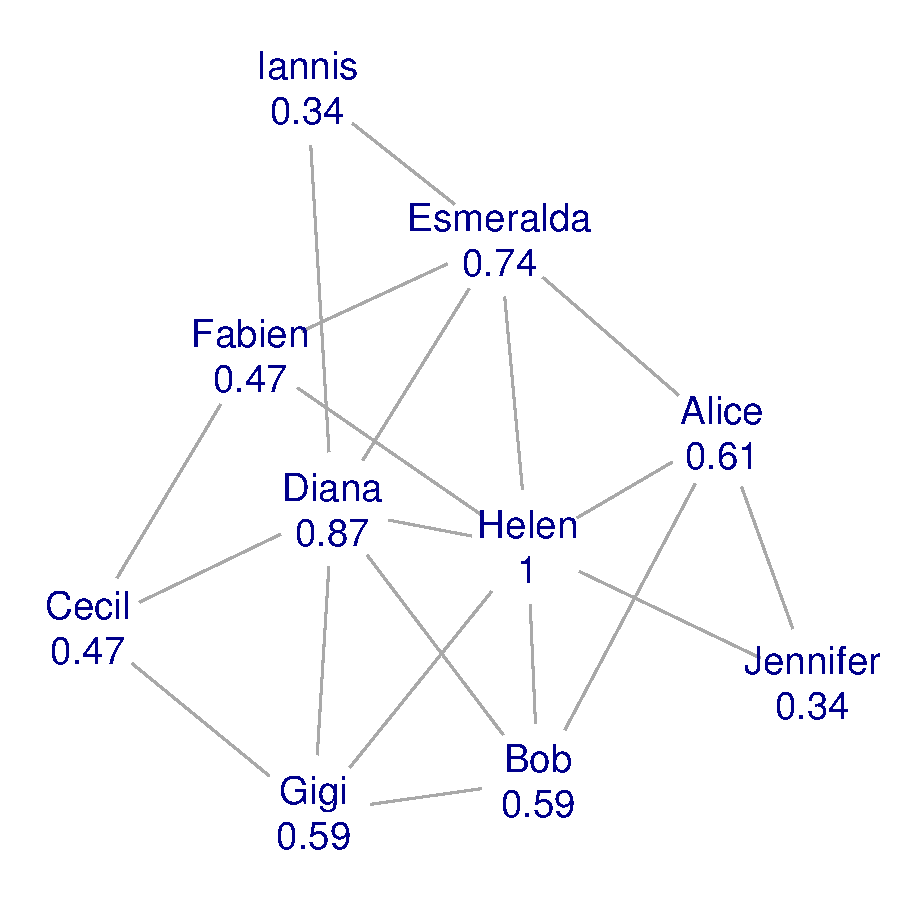
\includegraphics[width=0.45\textwidth]{ex-pagerank}
\end{center}
\end{itemize}
\end{narrow}

\newpage
\stitle{Community structure in networks}
\begin{narrow}{0cm}{15cm}
\begin{itemize}
\item Organizing things, clustering items to see the structure.
\begin{center}
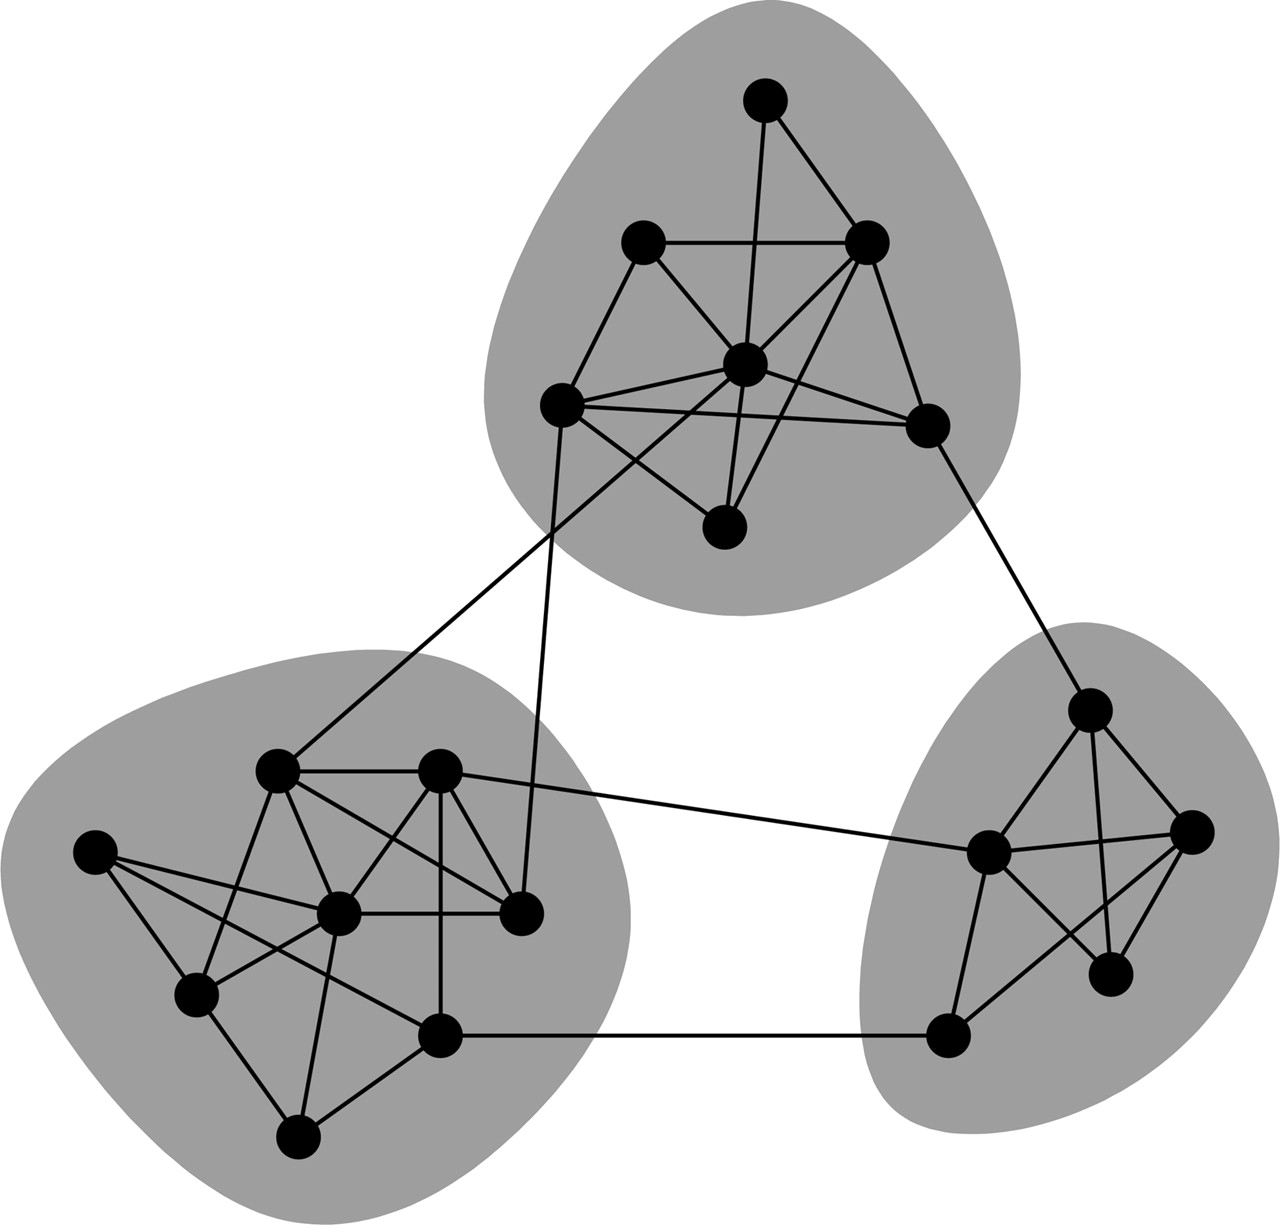
\includegraphics[width=0.45\textwidth]{commstr}\\[15pt]
{\tiny M. E. J. Newman, PNAS, 103, 8577--8582\par }
\end{center}
\end{itemize}
\end{narrow}

\newpage
\stitle{Community structure in networks}
\begin{narrow}{0cm}{15cm}
\begin{itemize}
\item How to define what is modular? Many proposed definitions, here
  is a popular one:
  \[ Q = \frac1{2|E|}\sum_{vw} [A_{vw} - p_{vw} ]\delta(c_v,c_w). \] \pause
\item Random graph null model: 
  \[ p_{vw} = p = \frac{1}{|V|(|V|-1)} \] \pause
\item Degree sequence based null model:
  \[ p_{vw} = \frac{k_vk_w}{2|E|} \]
\end{itemize}
\end{narrow}

% modularity, clustering, organizing things
% fast greedy
% betweenness
% spinglass

\newpage
\stitle{Cohesive blocks}
(Based on `Structural Cohesion and Embeddedness: a Hierarchical
Concept of Social Groups' by J.Moody and D.White, Americal
Sociological Review, 68, 103--127, 2003)

\begin{quotation}
Definition 1: A collectivity is structurally cohesive to the extent
that the social relations of its members hold it together. 
\end{quotation} \pause\vspace*{-0.8cm}

\begin{quotation}
Definition 2: A group is structurally cohesive to the extent that
multiple independent relational paths among all pairs of members hold
it together.
\end{quotation} \pause\vspace*{-0.8cm}

\begin{itemize}
\item Vertex-independent paths and vertex connectivity. \pause\vspace*{-0.8cm}
\item Vertex connectivity and network flows.
\end{itemize}

\newpage
\stitle{Cohesive blocks}
\vspace*{-3cm}
{\centering
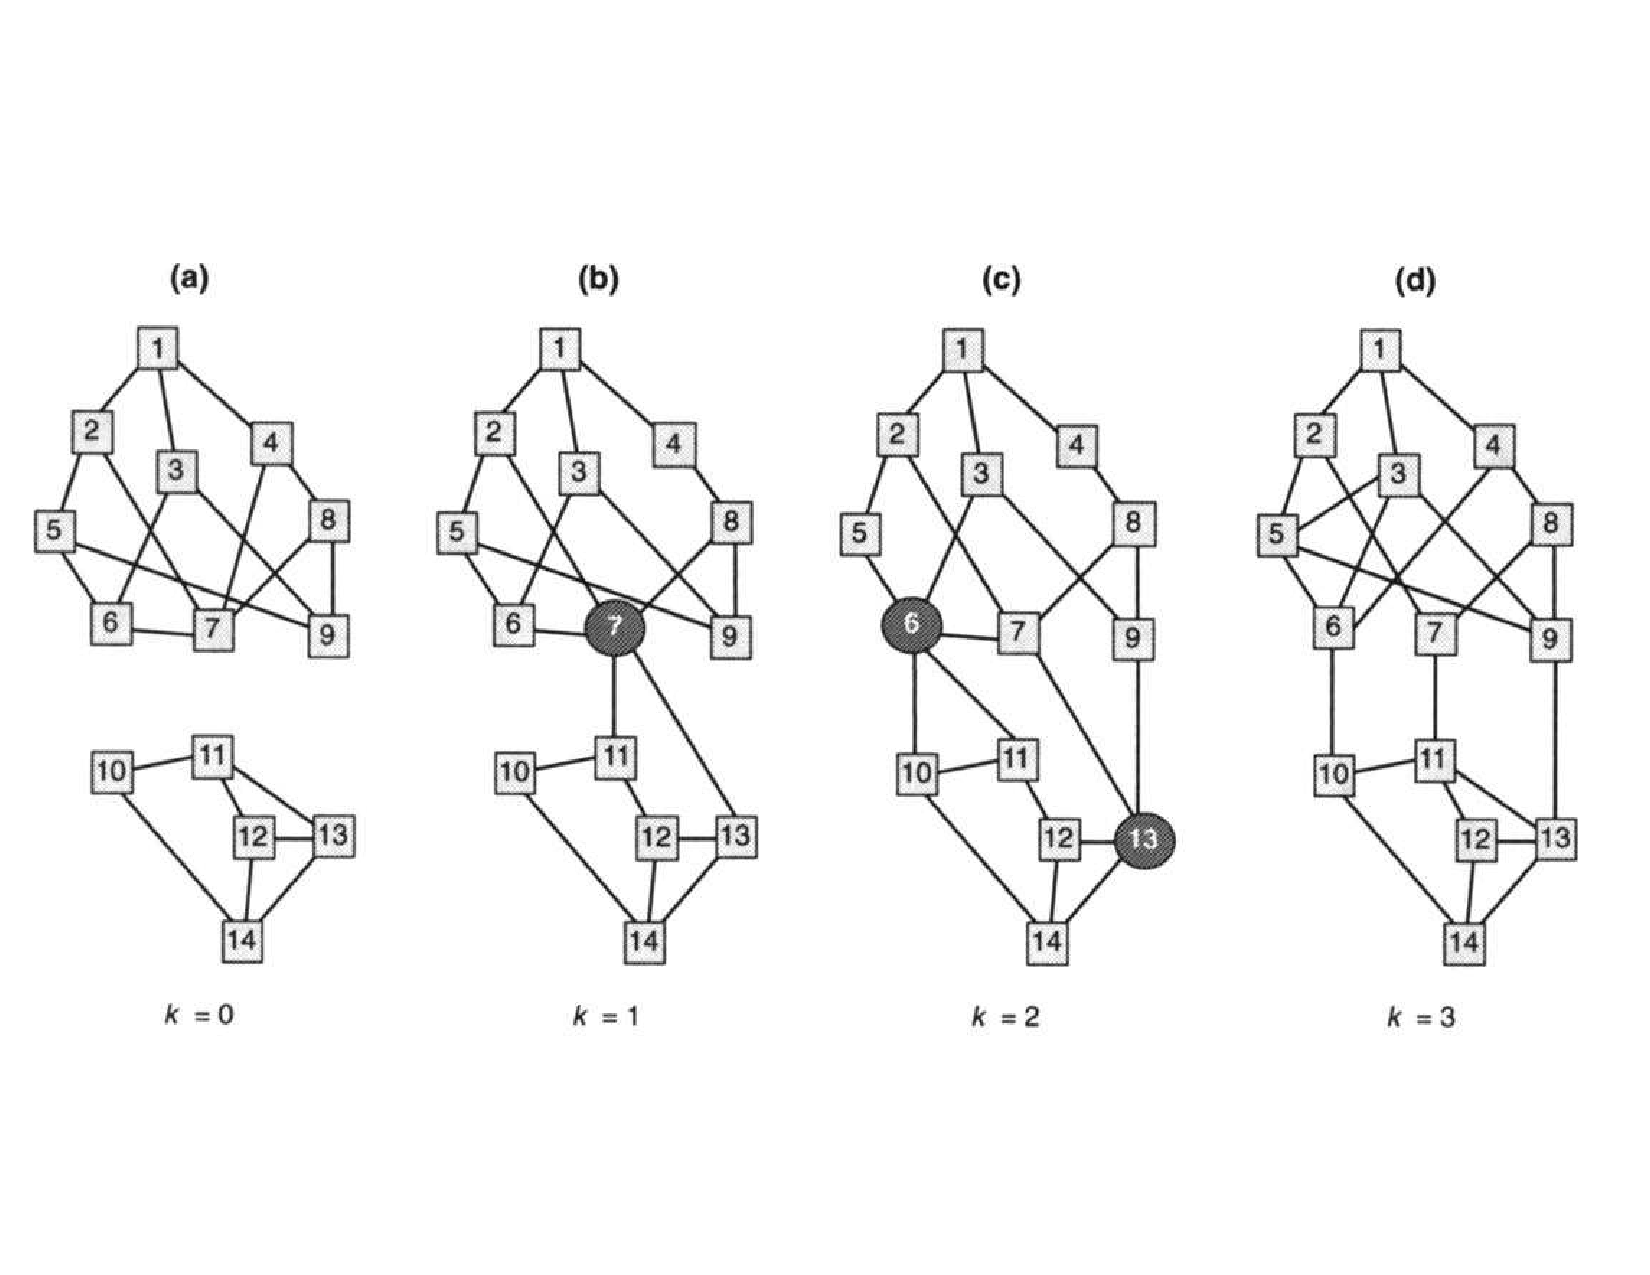
\includegraphics[width=0.9\textwidth]{groups}\\
}

\newpage
\stitle{Cohesive blocks}
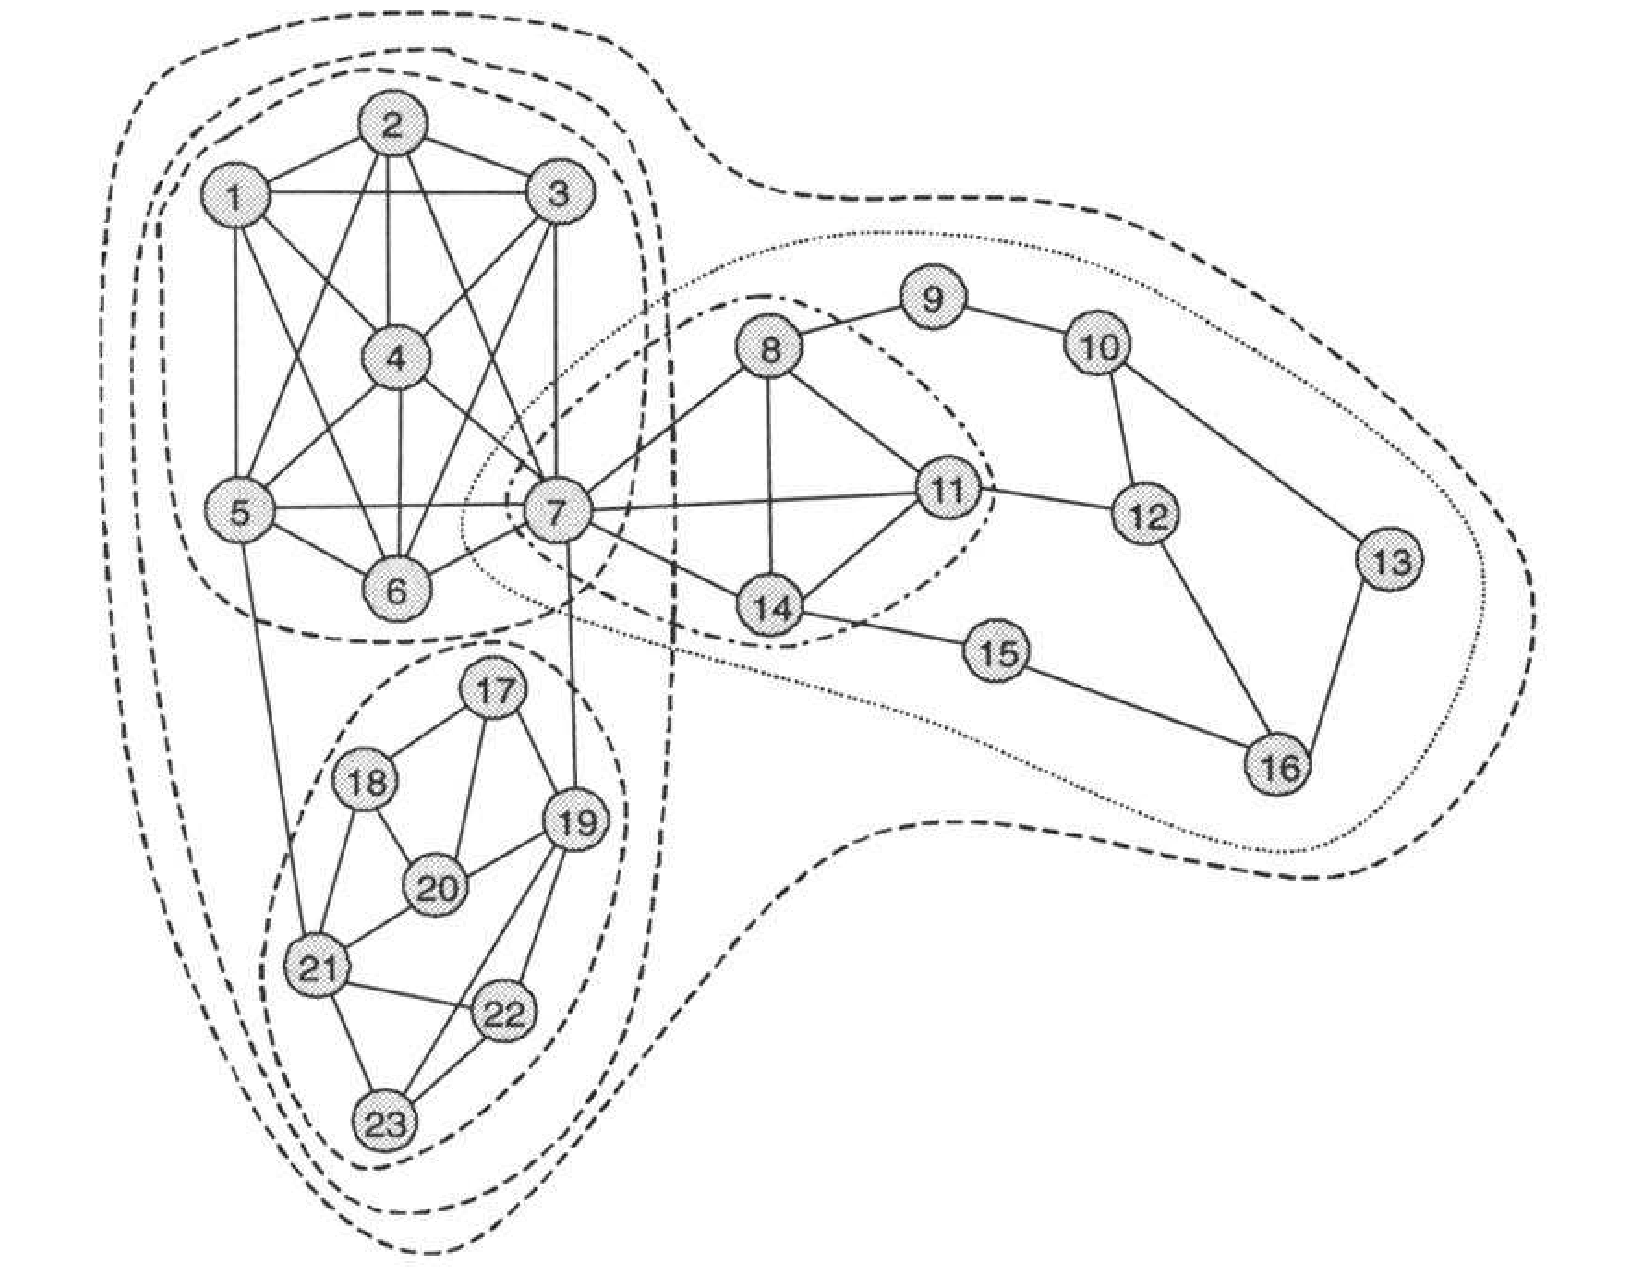
\includegraphics[width=0.6\textwidth]{cblocks}\\

\newpage
\stitle{Rapid prototyping}
\begin{narrow}{0cm}{15cm}
Weighted transitivity
\[ c(i)=\frac{\mathbf{A}^3_{ii}}{(\mathbf{A1A})_{ii}} \] \pause
\[ c_w(i)=\frac{\mathbf{W}^3_{ii}}{(\mathbf{WW_{\text{max}}W})_{ii}} \] \pause
\begin{Myverb}
  wtrans <- function(g) \{
    W <- get.adjacency(g, attr="weight")
    WM <- matrix(max(W), nrow(W), ncol(W))
    diag(WM) <- 0
    diag( W %*% W %*% W ) / 
       diag( W %*% WM %*% W)
  \}
\end{Myverb}
\end{narrow}

\newpage
\stitle{Rapid prototyping}
\begin{narrow}{0cm}{15cm}
Clique percolation (Palla et al., Nature 435, 814, 2005)
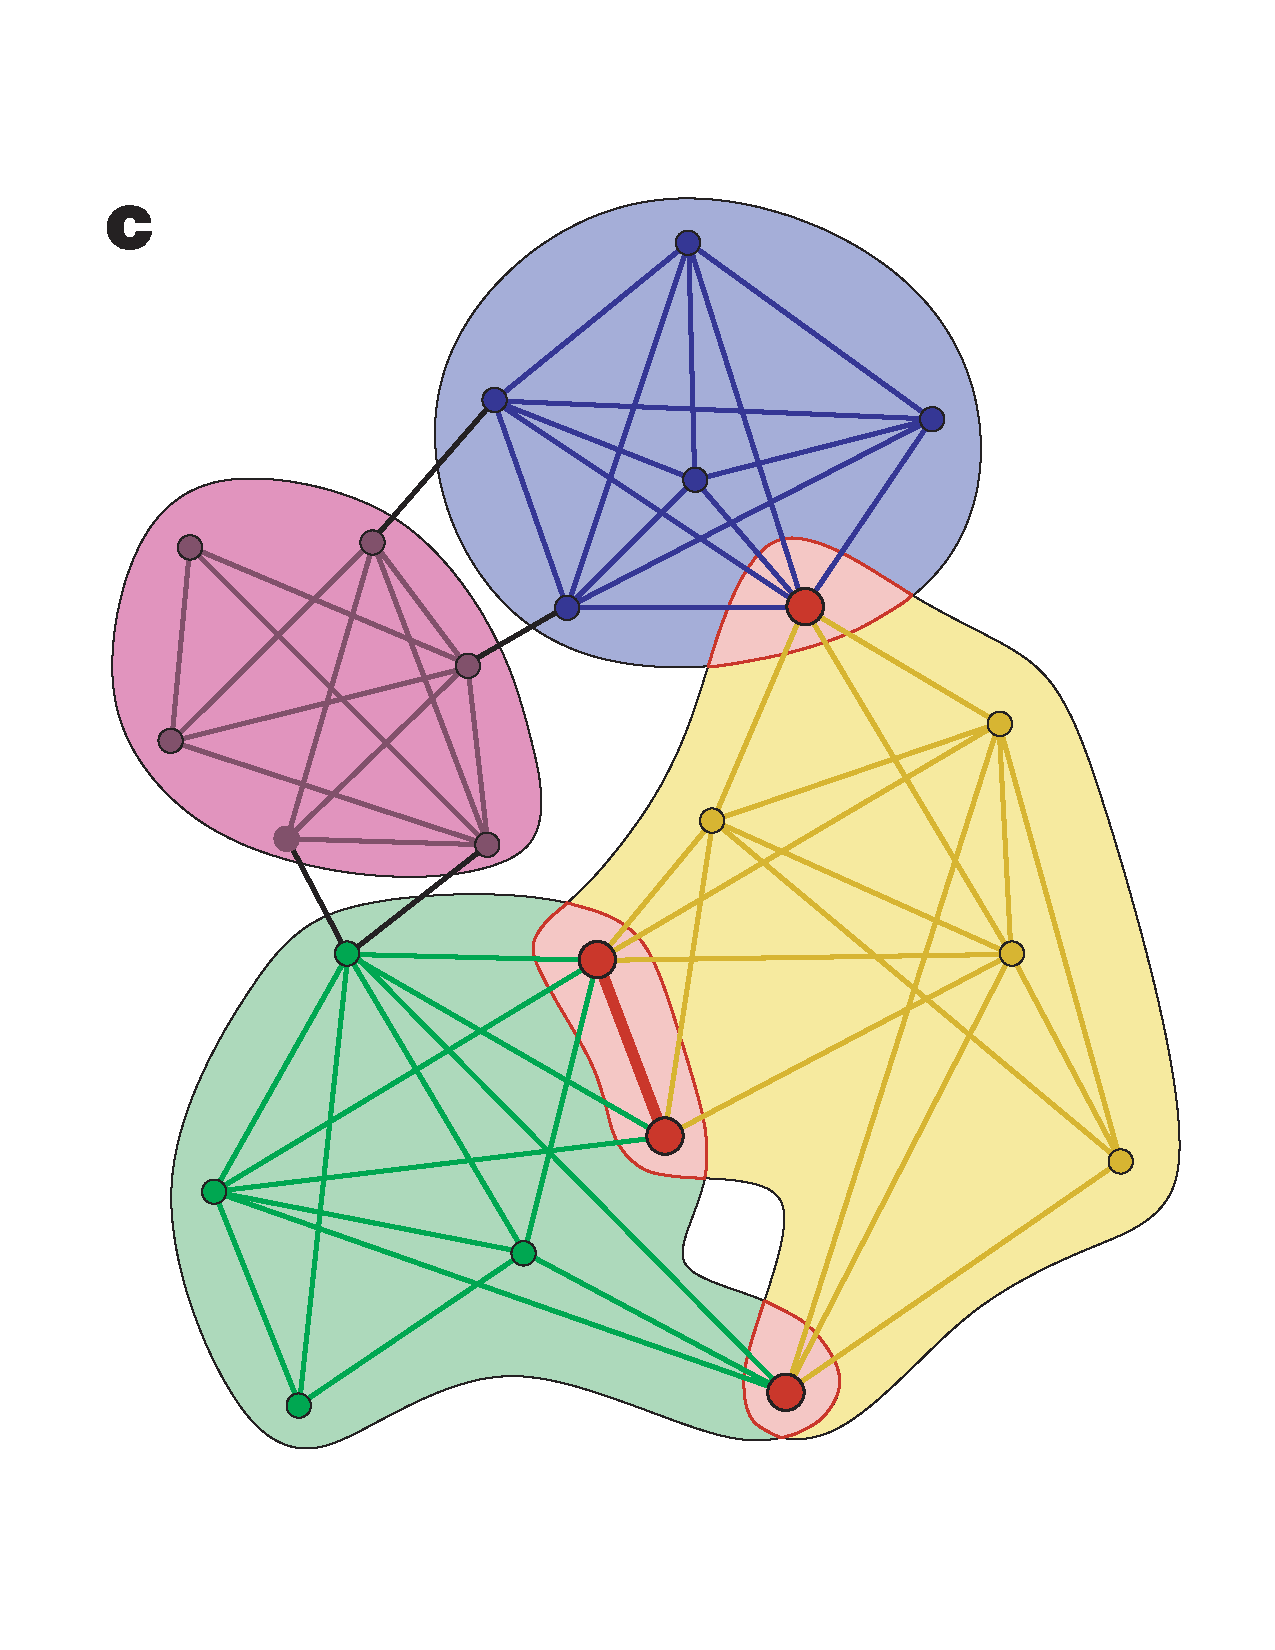
\includegraphics[width=0.4\textwidth]{vicsek}
\end{narrow}

\newpage
\stitle{\ldots and the rest}
\begin{narrow}{0cm}{15cm}
\begin{itemize}
\item Cliques and independent vertex sets.
\item Network flows.
\item Motifs, i.e. dyad and triad census.
\item Random graph generators.
\item Graph isomorphism.
\item Vertex similarity measures, topological sorting, 
  spanning trees, graph components, K-cores, transitivity or
  clustering coefficient.
\item etc.
\item C-level: rich data type library.
\end{itemize}
\end{narrow}

\newpage
\cstitle{Acknowledgement}

\begin{center}
\vfill
Tam\'as Nepusz\par\vfil
All the people who contributed code, sent bug reports, suggestions\par\vfil
The R project\par\vfil
Hungarian Academy of Sciences\par\vfil
The OSS community in general\par\vfill
\end{center}

\end{document}
